\documentclass{article}
\usepackage[utf8]{inputenc}
\usepackage{geometry}
\usepackage{longtable}
\usepackage{graphicx} % For including images
\usepackage{hyperref} % For hyperlinks
\usepackage{enumitem}
\usepackage{graphicx}
\usepackage{booktabs} % For professional looking tables
\usepackage{float} % For improved control over floating environments

\geometry{
 a4paper,
 total={170mm,257mm},
 left=20mm,
 top=20mm,
}

\title{Laboratory Assignment 1: Software Architecture of the Moon Climbing Application}
\author{Alessandro Combi}
\date{\today}

\begin{document}

\maketitle
\newpage

\tableofcontents
\newpage

\section{Software System}% add user required QAs

The MoonBoard is an innovative climbing training tool, allowing climbers to access a global database of climbing problems (routes) set on a standardized climbing wall with a grid of holds. 
Each problem can be lit up via LEDs under each hold, guided by a smartphone app that connects climbers worldwide, enabling them to try the same problems and share their progress. 
The smartphone app is called Moon Climbing.

Typical stakeholders of the system are climbers and climbing gym owners, or even private MoonBoard owners. 
MoonBoards come in a number of standards, set by inclination (40 or 25 degrees) and size (normal or mini) and can be bought and installed by anyone.

Typical requirements by the users can be summarized and related to Quality Attributes as follows:
\begin{itemize}
    \item \textbf{usability}: the application should provide a simple and usable interface for climbers around the world,
    \item \textbf{deployability}: it should be easy to provide new services and update the application, as of the current state the application doesn't have a good reputation among users,
    \item \textbf{integrability}: the application should be easily integrated with other systems, for instance global statistics trakers or gym websites,
    \item \textbf{modifiability}: the application should be modifiable, so that the functionalities can change to respond to the needs and feedback of the climbing community.
\end{itemize}    

\section{Components}\label{sec:components}
The functionalities of the moon boarding application can be summarized as a set of services that it deploys for the user:
\begin{itemize}
    \item User authentication,
    \item User interactions,
    \item Climbing problems insertion and retrieval,
    \item Users logbooks maintenance,
    \item Statistics and rankings tracking,
    \item Interaction with the physical board (to light up the appropriate LEDs),
    \item Update of user profiles.
\end{itemize}

Furthermore, the gyms are allowed to register their MoonBoards to the system, so that climbers can add information on which gym they climb. 
A ranking for gyms is also maintained.

A number of databases also need to be included in the system, such as the following:
\begin{itemize}
    \item Users logbooks, to archive which problems were solved by which user,
    \item Problems and boards archive,
    \item Gyms archive, each connected to a number of boards,
    \item User data storage.
\end{itemize}

\section{Deployment Models}\label{sec:models}

A suitable model can be a Public Cloud, like AWS, GCP, Microsoft Azure, with the nodes consisting in either serverless based processing nodes or serverless databases nodes (such as Amazon Aurora or Azure Cosmos DB). 
Serverless processing nodes should use Function as a Service (FaaS) to function, without having to explicitely allocate resources, not even to a virtual environment.

Function as a Service (FaaS) is a serverless computing concept that lets developers write functions that are triggered by events, are stateless and abstract from the infrastructure hosting them. The Cloud provider is tasked with the management of servers and can scale computational resources for a particular function according to the needs (typically the Events nature or their frequency).

In the following paragraphs, the benefits and drawback of applying FaaS are discussed, referring them to this particular system and to quality attributes.

\paragraph*{Benefits}
\begin{itemize}
    \item \textbf{Event Driven}: FaaS is consistent with Event Driven architectures. The Moon Climbing app seems suitable, since events can be represented by new climbing problems insertions, climbing problem solutions by a particular user, new boards design, etc. These are single occurrencies, rather than complex, real-time interactions.
    \item \textbf{Scalability}: The cloud provider automatically scales the execution of functions up or down based on the number of events or requests, handling many requests in parallel without manual intervention. Our app might need scaling of resources during climbing international competitions, where the sport popularity peaks, or during specific times of the day (typically after-work hours or after-dinner time in Europe or US, where it is mostly popular).
    \item \textbf{Cost efficiency}: Billing is based on the actual amount of resources consumed by executions of the functions, down to the level of milliseconds of execution time, rather than pre-provisioned capacity. Therefore, the cost of maintaining the system during hours of the day where no-one climbs in the major users geographical areas is very low.
    \item \textbf{Stateless}: Each function execution is stateless, with no knowledge of previous invocations. State needs to be stored externally, for example, in a database or a persistent storage service. Our services are mostly statistics insertion and retrieval, thus they seem perfectly suited for database storages.
\end{itemize}

\paragraph*{Drawbacks}
\begin{itemize}
    \item \textbf{Cold Starts}: Invoking a serverless function after it has been idle for some period can cause latency or delay. This delay is primarily due to the time it takes for the cloud provider to allocate resources, initialize the runtime environment, and start executing the function. In our application, slight delays can be considered acceptable.
    \item \textbf{Complexity}: Monitoring and debugging can be difficult compared to server-based architecture or monolithes. We deem this problem mitigated by the overall conceptual simplicity of the system as a whole. Bugs and malfunctioning are easier to individuate when interactions are limited by the scope of the system.
    \item \textbf{Vendor Lock-in}: Designing a FaaS might make switching cloud providers very hard, due to specific configurations, APIs, and behaviors. This is a problem that is really difficult to mitigate, given the asymmetrical nature of the relations with the Cloud Provider. We consider though that this is a drawback that is more than balanced by the many benefits listed.
\end{itemize}

Alternatives to this choice could include Private or Hybrid Cloud models, but we deem the data handled by the system not sensitive nor private enough to justify such a choice. 
Choosing physical servers or even virtual machines for such an application would require the prior knowledge and careful analysis of the requirements, which depends heavily on the time of the day and year, of the evolution in the popularity of the application and of the sport, and its fluctuations. The prediction of such variables is complex and not in the expertise of a developing team, which is a good reason for a highly flexible solution like a completely serverless model.

\section{Deployment Patterns and Styles}

\subsection{Microservices architecture}
Given the set of deployment nodes listed in Section \ref{sec:models}, it seems natural to employ a Microservices Architecture Pattern.
This design pattern structure the system as a set of independently deployable services the communicate only via service interfaces.

In the following paragraphs, the benefits and drawback of applying this pattern, referring them to this particular system.
\paragraph*{Benefits}
\begin{itemize}
    \item \textbf{Scalability}:
    Microservices allow each component of the Moon Climbing app, such as user authentication, problems management, and statistics tracking, to scale independently based on demand. This is particularly beneficial during peak usage times or as the app grows in popularity, ensuring that resources are efficiently allocated and the app remains responsive.    
    \item \textbf{Technological flexibility}:
    Each service might require different technologies that do not necessarily have to be compatible, given the choice of loose coupling between services. For instance, databases can have diffent technologies for different uses: those holding statistics and rankings should be relational DBs, known for their reliability and speed, given the structured nature of climbing problems log (each problem is well defined, it can be passed or not and a certain difficulty grade is assigned). Those holding user interactions could instead be noSQL, offering high schema flexibility, given the unstructured nature of this kind of data (images, videos, etc.).
    Furthermore, if real-time interaction with boards was offered (for instance to create competitions among many distant partecipants), this would require real-time processing capabilities, unlike statistics and logbooks calculations and retrieval.
    \item \textbf{Ease of Integration}
    This would also allow potential expansion of the architecture by external developers, for instance adding thier own special board with its specific allowed interactions.
    \item \textbf{Efficient resources utilization}
    A microservices architecture allows to allocate computational, memory and data resources efficiently across different services.
\end{itemize}

\paragraph*{Drawbacks}
\begin{itemize}
    \item \textbf{Performance Overhead}: microservices have to communicate via a network, which is slower than in-memory communication. In the Moon Climbing App case, it doesn't seem like this can be a major drawback, as it is used mostly to store and retrieve statistics and problems, which doesn't require for high speed. For this kind of problem, tactics like caching in memory stats and rankings with event-driven cache and DB updates should be sufficient. 
    \item \textbf{Cost of maintaining different technologies}: The flexibility explained above comes with a cost of maintaining different technologies and having expertise in managing them. This can be mitigated to an extent by using Cloud infrastructure, which allow part of the technological challenges to be moved to the Cloud provider.
    \item \textbf{Complexity}: designing and maintaining a microservices architecture is a complex effort, due to the number of connections and the number of services. In the context of the Moon Climbing app, the limited scale of the project seems small enough not to worry about this.
\end{itemize}

Following this discussion, we can list a set of microservices that the Moon Climbing App is made of. 
These services will be allocated each in their own environment and possibly in different machines (virtual or not).

\begin{itemize}
    \item \textbf{User authentication}: this service allow users to authenticate with their name, email, password and modify this data.
    \item \textbf{User interaction}: this service allow users to add other users as contact, check other users profiles.
    \item \textbf{Statistics and rankings}: this service allows users to check ranking in their region or globally, to check gym rankings or statistics on most popular problems.
    \item \textbf{Climbing Problems}: this service let users insert or retrieve climbing problems related to a particular version and setup of the moon board, which can be subsequently added to their logbook or to a favourite list, communicated to the statistics microservice, archived for other climbers use.
    \item \textbf{Physical Board software}: this is just a software that can interface with the climbers phone app via bluetooth, receive a problems data and light LED lights accordingly. In the future this could become a full-fledged service, allowing for a board interface, real-time problem sharing and perhaps network connection, instead of bluetooth.
\end{itemize}

\subsection{Database per Service}
As a consequence of choosing a microservices architecture is the loose coupling of services. Some services might require querying datas related with other services, and different services might require diffrent data storage methods.
The \textit{Database per Service} pattern solves these problem by prescribing the following:
\begin{itemize}
\item Keep each microservice's persistent data private to that service and accessible only via its API. A service's transactions only involve its database.
\end{itemize}

The service's database can be considered part of the implementation of that service. It cannot be accessed directly by other services.

This can be achieved for instance using one Database Server per Service.
Consistently with the choice of using serverless computing, we can also use serverless databases as mentioned in Section \ref{sec:models}.

\section{Deployment tactics}

In this Section tactics for managing the deployment pipeline and the deployed system are discussed.

\subsection{Deployment Pipeline tactic: Scale rollouts}[\textit{Related QA:  Deployability}]
This tactic involves deploying a new version of a service gradually, to a subset of the population rather than to the entire user base, without explicitely notifying them. As a consequence, the effect of the update can be monitored and in case rolled back. This ensures a lower impact when realising a malfunctioning or bugged update of a service. As such it can improve \textit{deployability} without sacrificing \textit{availability} and \textit{usability} for the whole user base.
It can also be used to collect feedback from the user experimenting the new version.

\subsection{Deployed System management tactic: Feature toggle}[\textit{Related QA: Deployability}]
This tactic consist of integrating a "kill switch" into the application, in order to deactived a feature in the system at runtime, without having to restart the deployment. It reliefs some of the responsibilities from testing.

\subsection{Encapsulation}[\textit{Related QA: Integrability}]
Encapsulation consist of having an explicit interface to an element and ensuring that any access to the element goes through the interface. It ensures internal parts of an element are not exposed and allows for similar elements to be seamlessy integrated in the system, provided that they implement the same interface. It also allows to expose different part of an element to different external accessors (if the element implements many interfaces).

\section{Deployment model}
\subsection{Deployment nodes}
In this Section we list the deployment nodes of the system. As discuss in the previous section, each service should have its own FaaS environment dedicated, and each one its corresponding database (one or more).
First the processing nodes are listed:
\begin{itemize}
    \item Problems FaaS environment: responsible for the insertion and retrieval of problems into the Database, it also supports filtering and querying,
    \item Problems and Logbooks DB Environment: keeping a set of climbing problems classified by type of board and level of difficulty, and the logbook of each user. Every time a new problem is solved by a climber and added to its logbook, a message needs to be sent the the Statistics environment, in order to record the stats. An alternative is to add an event-driven update process that only connects to the Logbooks database and the statistics database and update the second periodically using data from the first one (which receives insertion directed by users directly).
    \item Statistics FaaS environment: responsible for the calculation and retrieval of regional or global rankings and the calculation of custom statistics. It should be able to communicate with the Problems environment in case statistics about a specific problem or set of problems are required.
    \item Statistics DB Environment: recording main rankings and statistics.
    \item User authentication FaaS environment.
    \item User data DB environment: keeps user authentication information, should be a secured database.
    \item User interaction FaaS environment: handles contacts, images retrieval	from Instagram or other socials (a climber can tag the application and the image is linked to a particular climbing problem), consulting of other climbers profiles.
    \item Profiles Data DB Environment: contains user profiles public data, such as their region and main statistics and rankings.
    \item Profile Update FaaS Environment: updates profiles rankings when the statistics environment receives new data.  
\end{itemize}

The client nodes can be the following:
\begin{itemize}
    \item Phone: hosting the application.
    \item Physical Board: containing a little device receiving via bluetooth from the users phone and lighting LEDs accordingly.
    \item Laptops: the application can also be accessed by laptop, also from Gyms.
\end{itemize}

\subsection{Deployment diagram}

The list of elements in the below diagram is in the previous section. The requirements of the environments are not listed, as they are able to scale according to needs and are handled directly by the cloud provider.
While infrastructure is managed by the cloud provider, some function configurations are needed in FaaS, such as:
\begin{itemize}
    \item memory allocation,
    \item execution timeouts,
    \item environment variables,
    \item runtime environments,
    \item event triggers: these can be database changes, HTTP requests, etc.
\end{itemize}

OS minimum requirements are considered for the smartphones hosting the app.

\begin{figure}[H]
    \centering
    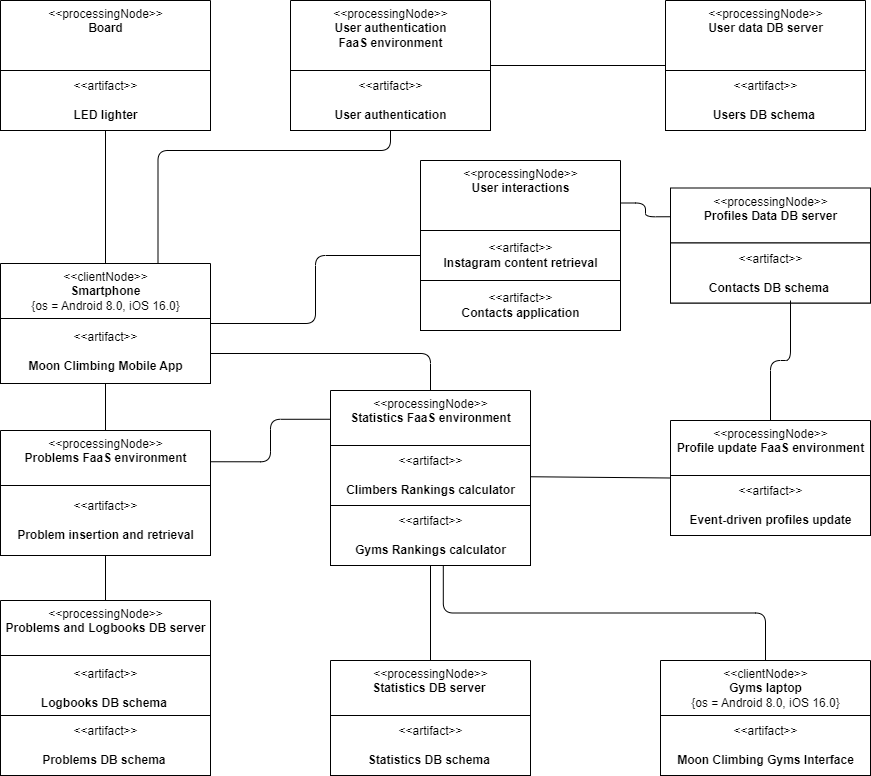
\includegraphics[width=\textwidth]{deployment_UML.png}
    \caption{Runtime platform model of the Moon Climbing Application.}
    \label{fig:trip_system}
\end{figure}

\end{document}